\documentclass{article}
	\pagestyle{plain}
	\usepackage{amsmath} % Required for some math elements 
	\usepackage[utf8]{inputenc}
	\usepackage{placeins}
	
	\usepackage[usenames,dvipsnames,svgnames,table]{xcolor}
	\usepackage{tikz-timing}[2009/05/15]
	\usepackage{multicol}
	\usepackage[T2A]{fontenc}
	\usepackage[russian]{babel}
	\usepackage[left=2.5cm, right=1.5cm, vmargin=2.5cm]{geometry}
	\setlength\parindent{0pt} % Removes all indentation from paragraphs

	\usepackage{listings} %% собственно, это и есть пакет listing
	\usepackage{caption}
	\DeclareCaptionFont{white}{\color{white}} %% это сделает текст заголовка 
	\DeclareCaptionFormat{listing}{\colorbox{gray}{\parbox{\textwidth}{#1#2#3}}}
	\captionsetup[lstlisting]{format=listing,labelfont=white,textfont=white}
	\renewcommand\labelenumi{\theenumi)}	
	
	\lstset{ %
		language=C++,                 % выбор языка для подсветки (здесь это С)
		basicstyle=\small, % размер и начертание шрифта для подсветки кода
		numbers=left,               % где поставить нумерацию строк (слева\справа)
		numberstyle=\tiny,           % размер шрифта для номеров строк
		stepnumber=1,                   % размер шага между двумя номерами строк
		firstnumber=1,
		numberfirstline=true
		numbersep=5pt,                % как далеко отстоят номера строк от подсвечиваемого кода
		backgroundcolor=\color{white}, % цвет фона подсветки - используем \usepackage{color}
		showspaces=false,            % показывать или нет пробелы специальными отступами
		showstringspaces=false,      % показывать или нет пробелы в строках
		showtabs=false,             % показывать или нет табуляцию в строках
		frame=single,              % рисовать рамку вокруг кода
		tabsize=2,                 % размер табуляции по умолчанию равен 2 пробелам
		captionpos=t,              % позиция заголовка вверху [t] или внизу [b] 
		breaklines=true,           % автоматически переносить строки (да\нет)
		breakatwhitespace=false, % переносить строки только если есть пробел
		escapeinside={\%*}{*)}   % если нужно добавить комментарии в коде
	}
	
\begin{document}

	%----------------------------------------------------------------------------------------
	%	TITLEPAGE 1
	%----------------------------------------------------------------------------------------		
	\begin{titlepage}
		\center 
		ФЕДЕРАЛЬНОЕ ГОСУДАРСТВЕННОЕ АВТОНОМНОЕ ОБРАЗОВАТЕЛЬНОЕ УЧЕРЕЖДЕНИЕ ВЫСШЕГО ОБРАЗОВАНИЯ\linebreak  
		«Санкт-Петербургский политехнический университет Петра Великого»\\[2cm]
		\textsc{\Large Институт компьютерных наук и технологий}\\[6.5cm]
		
		{\huge \bfseries Лабораторная работа №1\\[0.4cm]
			\Large \mdseries “Получение базовой последовательности псевдослучайных чисел и тестовые проверки его работы”}\\[6.5cm]
		
		\begin{multicols}{2}
			\begin{flushright} \large
				
				{Выполнил:}\\[0.5cm]
				
				{Проверил:}
				
			\end{flushright}
			\begin{flushright}
				
				{Каргалов Л.А.}\\[0.5cm]
				
				{Чуркин В. В.}
				
			\end{flushright}
		\end{multicols}

		\flushright{
			{\today}\\[0.5cm]
		}
		\centering{
			Санкт-Петербург\\
			\the\year
		}
		
		\vfill % Fill the rest of the page with whitespace
	\end{titlepage}
	
	%----------------------------------------------------------------------------------------
	%	TEBLE OF CONTENTS 1
	%----------------------------------------------------------------------------------------
	\tableofcontents
	\setcounter{page}{2}
	\newpage
	
	%----------------------------------------------------------------------------------------
	%	SECTION 1
	%----------------------------------------------------------------------------------------
	\section{Цель работы}
	\begin{enumerate}
	\item Получение на ЭВМ с помощью программного датчика
	базовой последовательности псевдослучайных чисел,
	имеющих равномерное распределение.
	\item Освоение методов статистической оценки полученного
	распределения: вычисление эмпирических значений
	для математического ожидания и дисперсии.
	\item Освоение методов оценки статистики связи: вычисление
	значений автокорреляционной функции и построение
	коррелограммы.
	\item Освоение методов графического представления законов
	распределения: построение функции плотности 
	распределения и интегральной функции распределения.
	\end{enumerate}
	
	\newpage
	
	%----------------------------------------------------------------------------------------
	%	SECTION 2
	%----------------------------------------------------------------------------------------
	\section{Ход работы}
	\begin {enumerate}
		\item С помощью программного датчика получены псевдослучайные числа $u[1],u[2],... u[n]$, имеющие равномерный характер распределения. Поставим  задачу простейшей оценки качества полученного датчика путем вычисления так называемых эмпирических точечных оценок распределения, в частности, математического ожидания и дисперсии, и сравнения полученных результатов с известными теоретическими значениями.
		\item Оценка  степени связанности псевдослучайных чисел определена с помощью корреляционной (или "автокорреляционной") функции $K(f)$ (построены кореллограммы), которая представляет собой последовательность коэффициентов корреляции, зависящих от величины сдвига $f$, как от аргумента.
		\item Приведено графическое представление законов распределения: построение эмпирической функции плотности распределения и эмпирической интегральной функции распределения и сравнение с соответствующими теоретическими кривыми.
	\end{enumerate}
	
	%------------------------------------------------------------
	%	SUBSECTION 1
	%------------------------------------------------------------
	\subsection{Результаты}
		\begin{enumerate}
			\item Таблица точечных оценок\\
				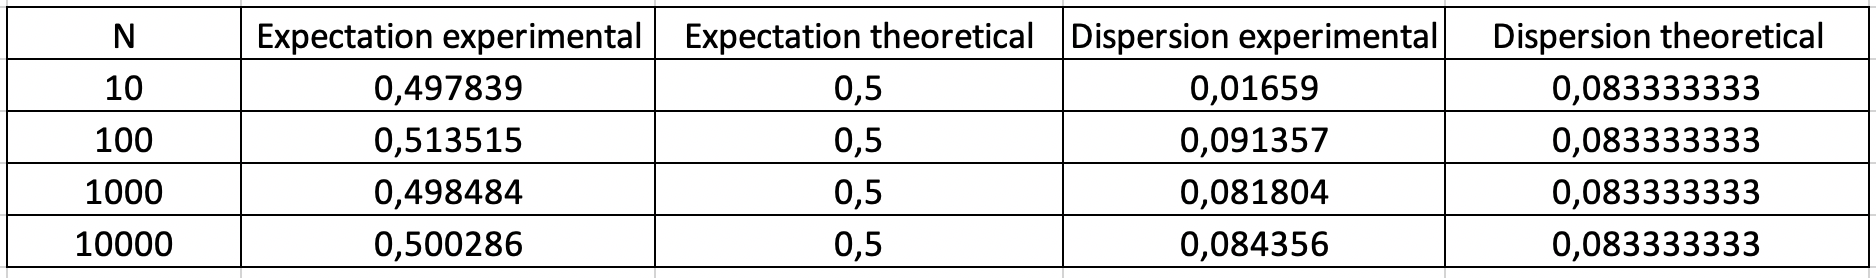
\includegraphics[scale=0.5]{table.png}
			
			\item График функции распределения\\
				\begin{figure}[!htb]
					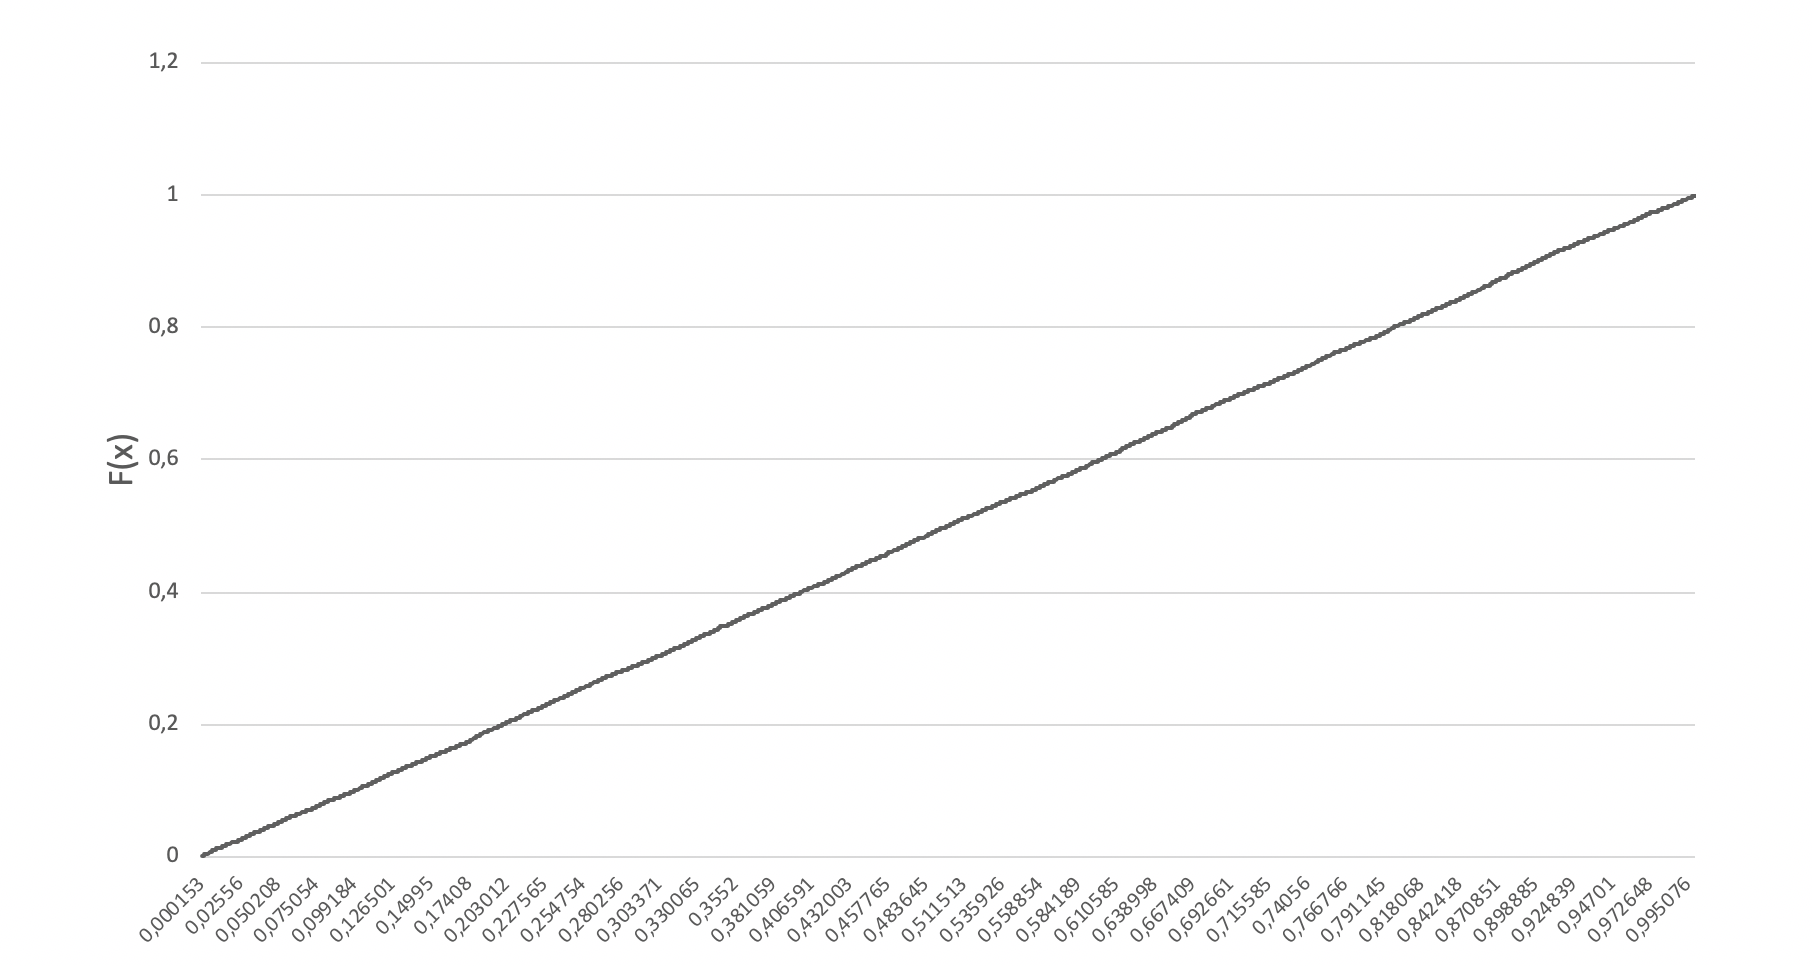
\includegraphics[scale=0.5]{6.png}
					\caption{Для $n = 10000$}
				\end{figure}

			\item График функции плотности распределения\\
				\begin{figure}[!htb]
					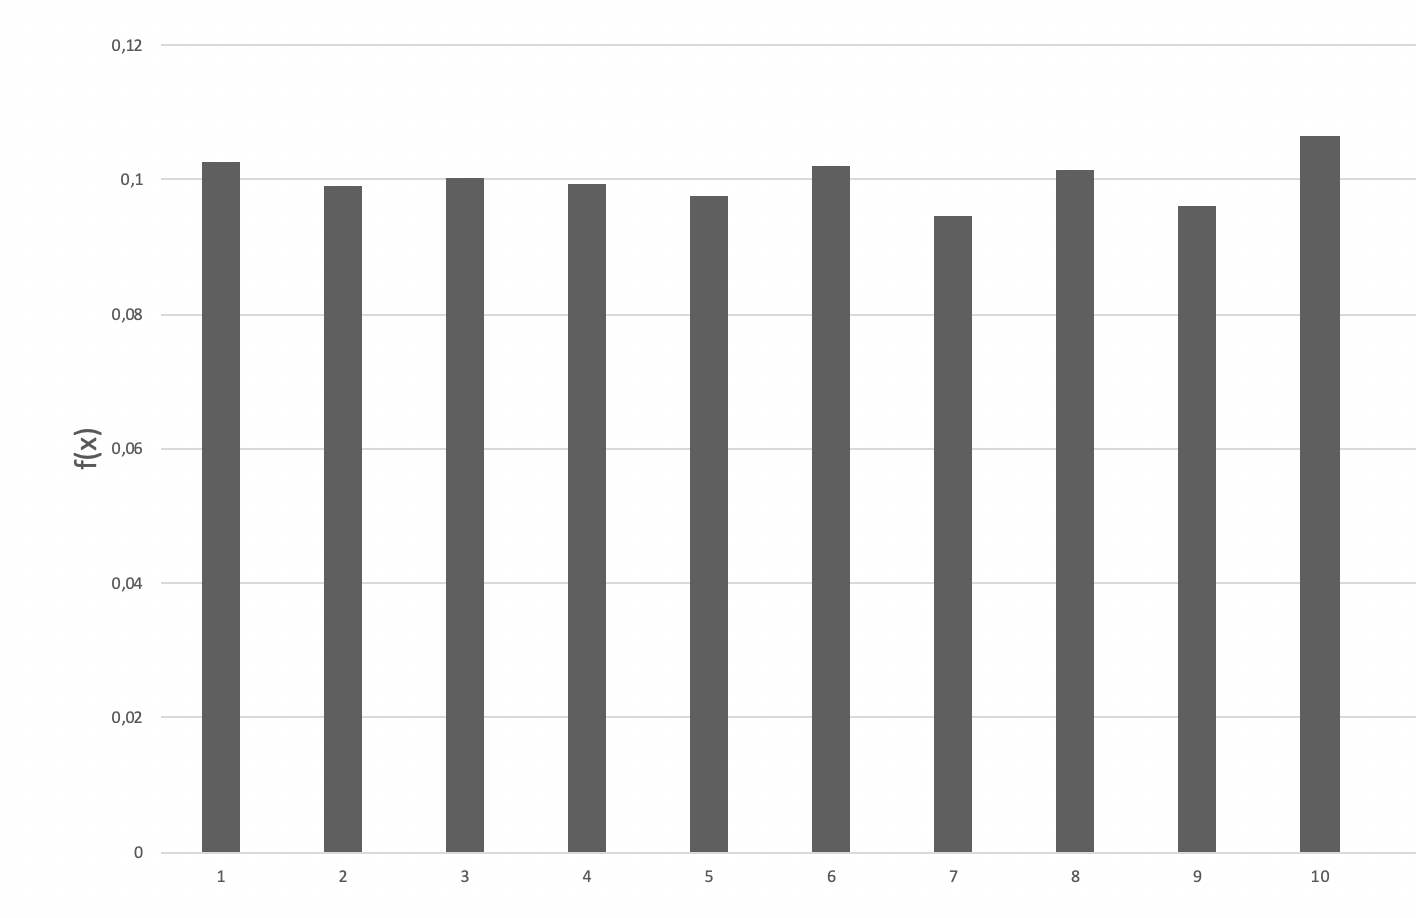
\includegraphics[scale=0.6]{5.png}
					\caption{Для $n = 10000$}
				\end{figure}
				
			\item Корелограммы\\
				\begin{figure}[!htb]
					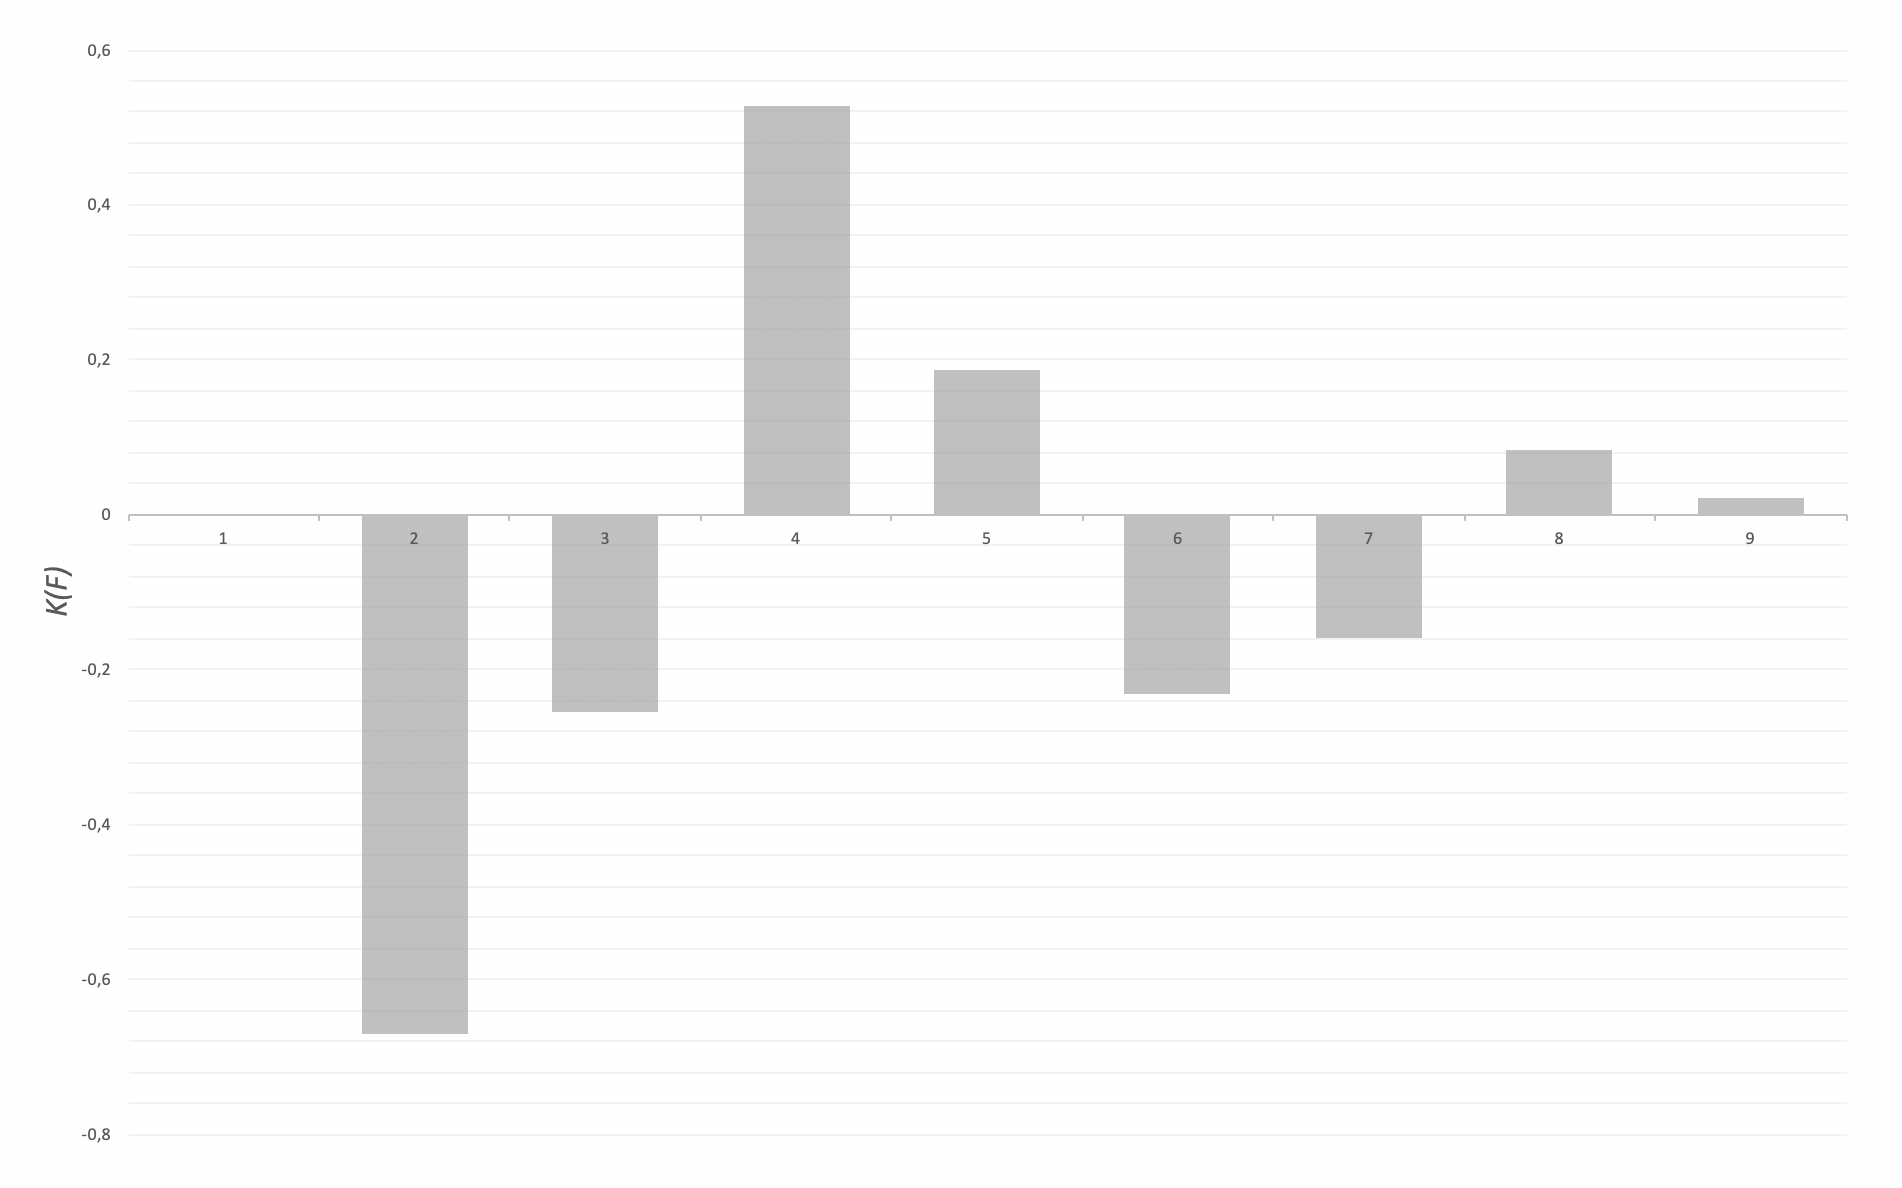
\includegraphics[scale=0.35]{1.png}
					\caption{Для $n = 10$}
				\end{figure}
				
				\begin{figure}[!htb]
					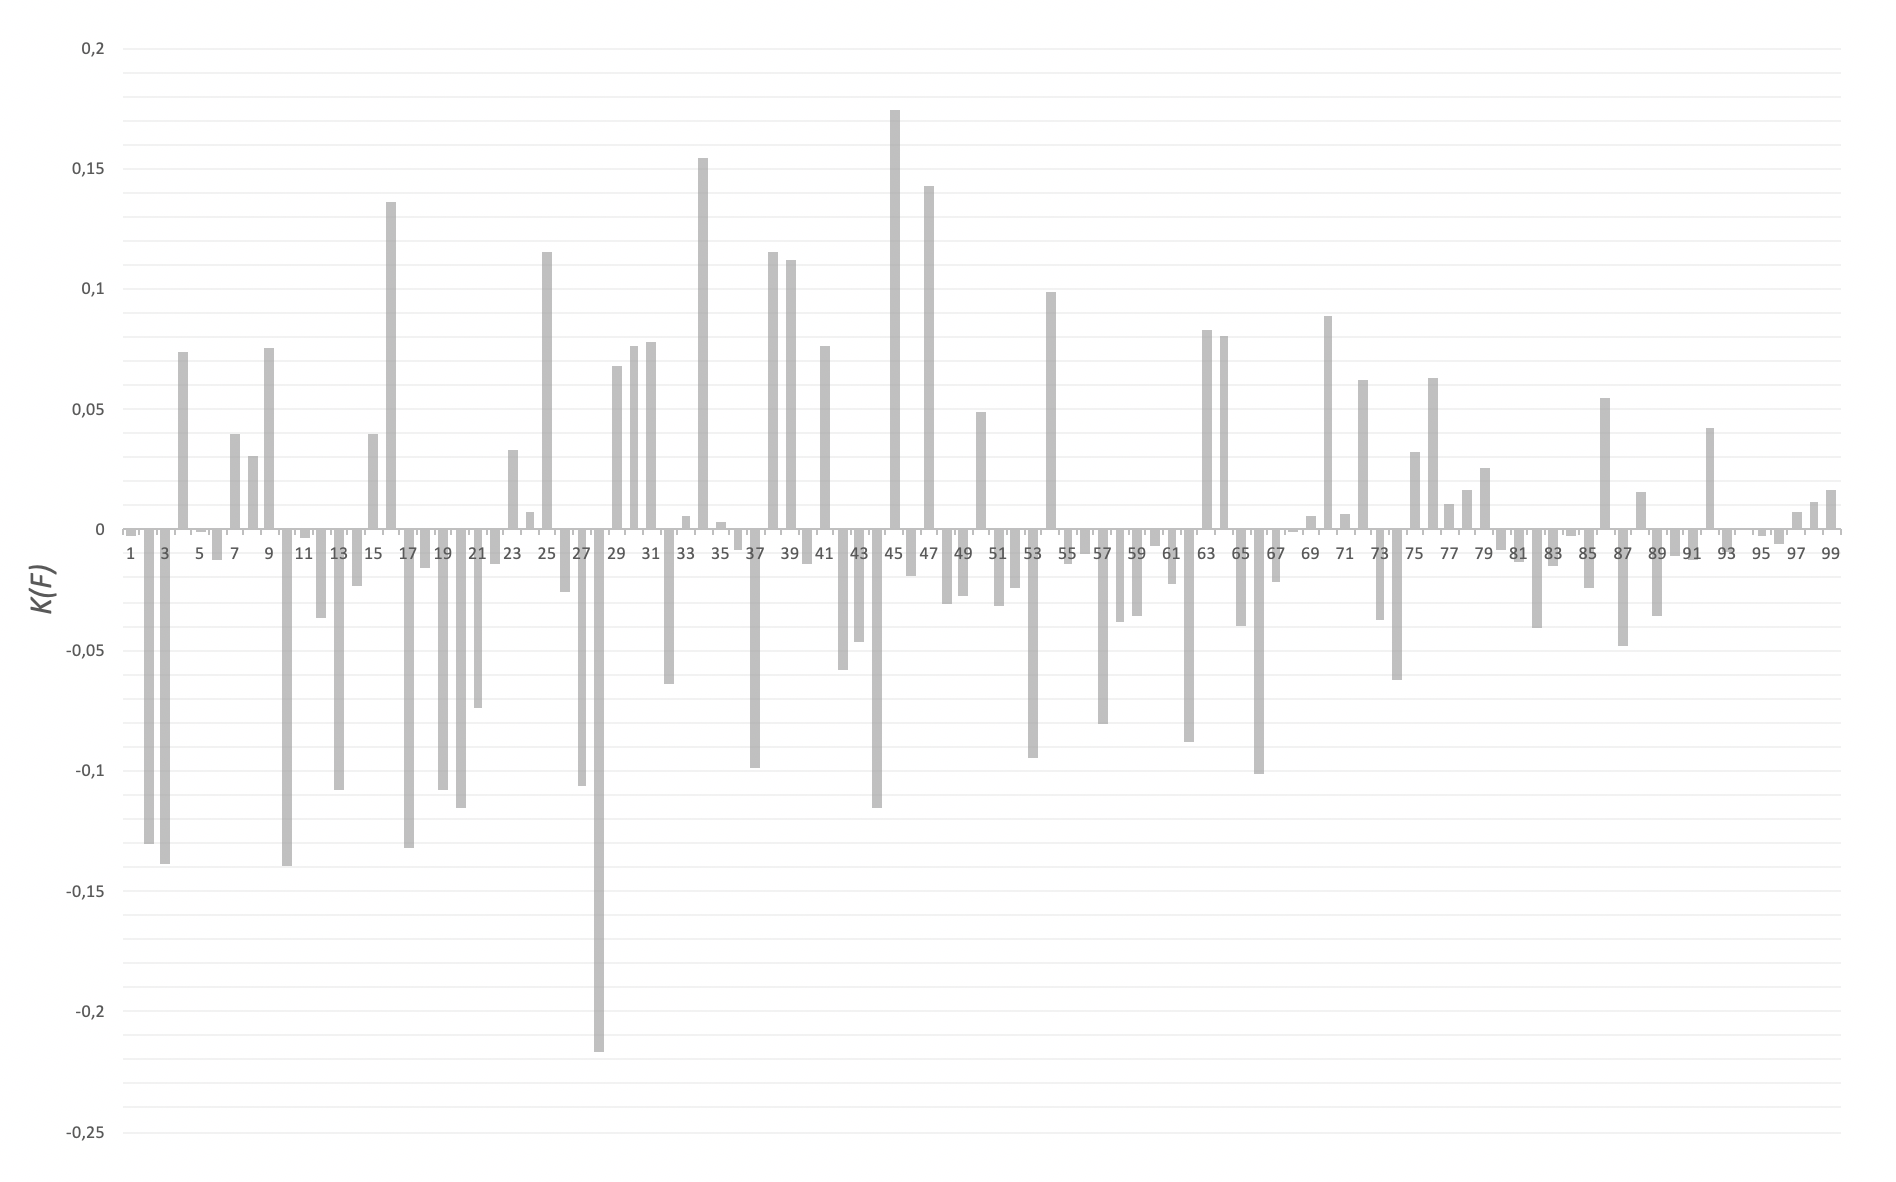
\includegraphics[scale=0.35]{2.png}
					\caption{Для $n = 100$}
				\end{figure}
				
				\begin{figure}[!htb]
					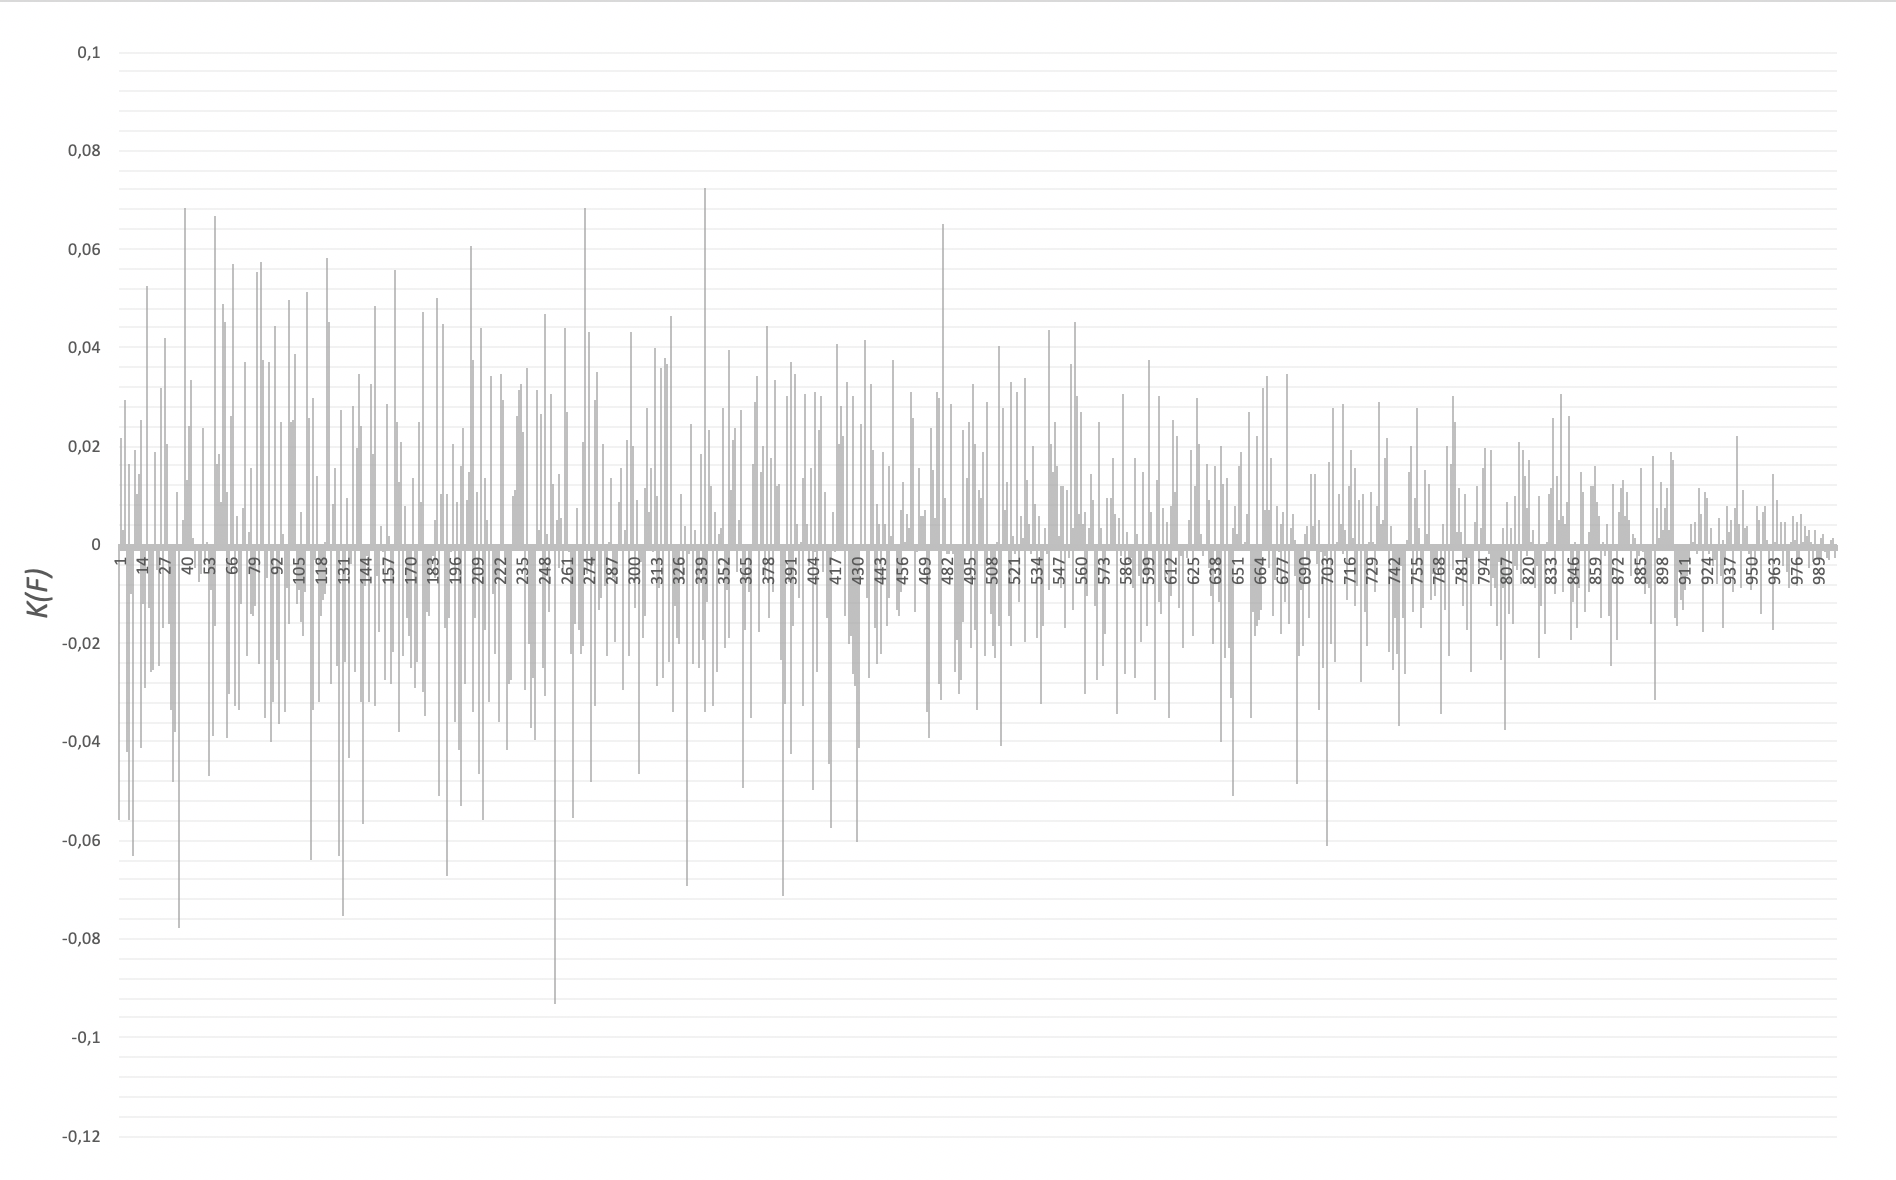
\includegraphics[scale=0.4]{3.png}
					\caption{Для $n = 1000$}
				\end{figure}
				
				\begin{figure}[!htb]
					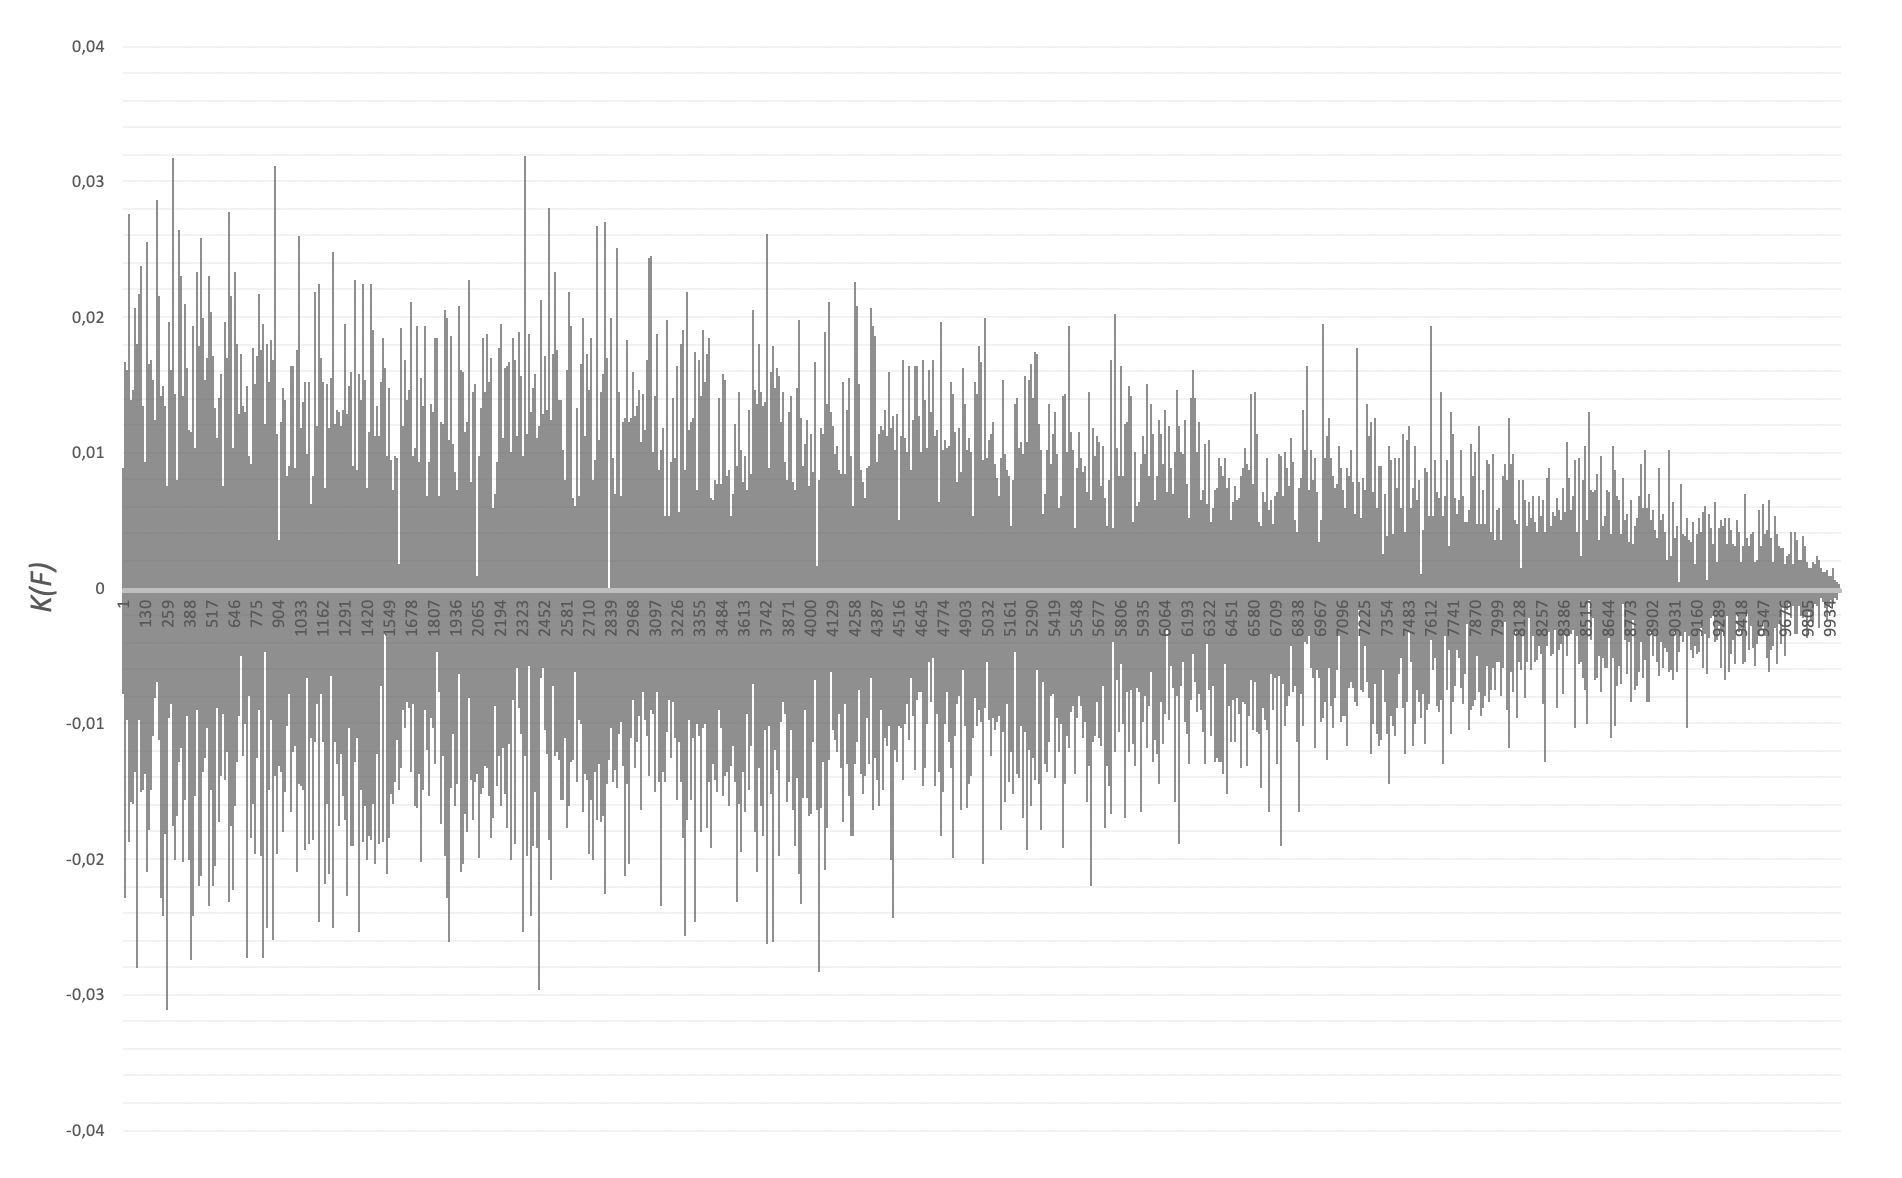
\includegraphics[scale=0.4]{4.png}
					\caption{Для $n = 10000$}
				\end{figure}		
		\end{enumerate}
	\FloatBarrier
	
	\clearpage
	\newpage
		
	%----------------------------------------------------------------------------------------
	%	SECTION 3
	%----------------------------------------------------------------------------------------
	\section{Выводы}
	Исходя из полученных точечных оценок, можно сказать, что при достаточно больших $n > 100$ значения математического ожидания и 
	дисперсии принимают значения соответствующие теоретическим, с некоторой погрешностью, это объясняется тем что с ростом размера 
	выборки полученные эмпирическим путем данные все лучше описывают теоретические.\\
	Так же, основываясь на графиках АКФ, можно сказать, что между элементами случайной последовательности существуют некоторые зависимости, 
	т.к. в точках не кратных $n$ значения АКФ не стремятся к нулю, еще можно заметить что график АКФ не имеет переодически повторяющихся 
	паттернов, что свидетельствует об отсутствии периодичности в исходной функции генератора. \\
	Поэтому встроенный класс $std::uniform\_real\_distribution<>$ можно использовать в качестве базового для получения псевдослучайных 
	величин с равномерным законом распределения.

	\newpage
	%------------------------------------------------------------
	%	Section 1
	%------------------------------------------------------------
	\section{Приложение}
	\subsection{Исходный код на языке С++}
	\lstinputlisting[caption = model.hpp]{../../src/labs/lab1/model.hpp}
	\lstinputlisting[caption = writer.hpp]{../../src/labs/lab1/writer.hpp}
	\lstinputlisting[caption = main.cpp]{../../src/labs/lab1/main.cpp}

		
\end{document}